%
%===============>>  ГРУППА 11-6 МОДУЛЬ 8  <<=============
%
\setmodule{Вспомнить всё}

%BEGIN_FOLD % ====>>_____ Занятие 1 _____<<====
\begin{class}[number=1]
	\begin{listofex}
		\item Решите уравнения: %5.30 5.32(о ф ь)
		\begin{tasks}(2)
			\task \( 0,6x-5,4=-0,8+5,8 \)
			\task \( \dfrac{5x}{6}+16=\dfrac{4}{9}x+9 \)
			\task \( \mfrac{2}{2}{5}x+ \mfrac{3}{2}{15}=\mfrac{3}{1}{5}x + \mfrac{2}{1}{3} \)
			\task \( \dfrac{3,6}{0,2(6y+1)}=\dfrac{9}{0,5y} \)
		\end{tasks}
		\item Решите уравнения:
		\begin{tasks}(1)
			\task \( (6x-2)(1-x)=-(3x+5)(2x-0,5) \)
			\task \( (3x+4)^2=(3x-5)(2+3x) \)
		\end{tasks}
		\item Вычислить:
		\begin{tasks}(2)
			\task \( \sqrt{1,44\cdot0,04\cdot0,0001} \)
			\task \( \sqrt{\dfrac{9}{16}\cdot\dfrac{4}{81}\cdot\dfrac{36}{169}} \)
			\task \( \sqrt{3}\cdot\sqrt{5}\cdot\sqrt{15} \)
			\task \( \sqrt{21\cdot65\cdot39\cdot35} \)
		\end{tasks}
		\item Упростить:
		\begin{tasks}(2)
			\task \( 13\sqrt{7}-2\sqrt{7}+5\sqrt{7} \)
			\task \( 19\sqrt{8}-6\sqrt{8}+12\sqrt{8} \)
			\task \( 4,6\sqrt{5}-2,5\sqrt{5}+0,2\sqrt{45} \)
			\task \exercise{1630}
		\end{tasks}
		\item Решите уравнения: %придуманные (117)
		\begin{tasks}(2)
			\task \( (x+9)(x+23)=0 \)
			\task \( x(-x-9,3)(-11+x)=0 \)
			\task \( 9x^2-18x+9=0 \)
		\end{tasks}
		\item Решите уравнения:
		\begin{enumcols}[itemcolumns=3]
			\item \exercise{386}
			\item \exercise{390}
			\item \exercise{401}
			\item \exercise{415}
		\end{enumcols}
		\item Решите уравнения:
		\begin{enumcols}[itemcolumns=2]
			\item \( 2x^2-5x-3=0 \)
			\item \( -2x^2=7x-9 \)
		\end{enumcols}
		\item Решите уравнение:
		\[6(x^2-3)^2+5(x^2-3)+6=0\]
		\item Найдите два числа, если их сумма равна \( 36 \), а произведение \( 315 \).
		\item Найдите число, зная, что прибавив к его квадрату \( 108 \), получим число в \( 24 \) раза больше данного.
	\end{listofex}
\end{class}
%END_FOLD

%BEGIN_FOLD % ====>>_ Домашняя работа 1 _<<====
\begin{homework}[number=1]
		\begin{listofex}
			\item Домашняя работа
		\end{listofex}
\end{homework}
%END_FOLD

%BEGIN_FOLD % ====>>_____ Занятие 2 _____<<====
\begin{class}[number=2]
	\begin{listofex}
		\item В прямоугольном треугольнике два катета равны \( 3 \) и \(  4 \). Найдите гипотенузу.
		\item В прямоугольном треугольнике гипотенуза равна \( 20 \), а один из катетов равен \( 12 \). Чему равен другой катет?
		\item Основание равнобедренного треугольника равно \( 16 \), боковая сторона равна \( 10 \). Чему равна высота проведенная к основанию этого треугольника?
		\item В прямоугольном треугольнике \( \angle C=90\degree \), \( AB=8 \), \( \angle A=30\degree \). Найдите угол \( B \). Чему будет равен катет \( CB \)?
		\item В прямоугольном треугольнике \( ABC \) катет \( AС \) равен половине гипотенузы \( AB \). Найдите градусную меру всех углов треугольника.
		\item Известно, что в прямоугольном треугольнике (\( \angle C=90\degree \)) угол \( B=60\degree \). Найдите прилежащий к этому углу катет, если гипотенуза равна \( 50 \).
		\item В треугольнике \( ABC \) высота \( CD=15 \), \( AB=22 \). Найдите площадь треугольника \( ABC \).
		\item Периметр треугольника \( ABC \) равен \( 14 \), \( AB=6 \), \( BC=5 \). Высота \( BH=4 \). Найдите площадь треугольника.
		\item Периметр равнобедренного треугольника равен \( 16 \), а боковая сторона --- \( 5 \). Найдите площадь треугольника.
		\item В параллелограмме \( ABCD \) два противоположных угла в сумме равны \( 140\degree \). Найдите два других угла.
		\item В параллелограмме \( ABCD \) одна сторона в два раза больше соседней стороны. Найдите длины сторон параллелограмма \( ABCD \), если его периметр равен \( 36 \).
		\item Биссектриса угла параллелограмма делит его сторону на отрезки \( 3 \) и \( 4 \). Найдите стороны параллелограмма.
		\item В параллелограмме \( ABCD \) проведены биссектрисы из вершин \( A \) и \( B \), которые пересекаются в точке \( O \). Чему равен угол \( \angle AOB \), если \( \angle B= 40\degree \)?
		\item Диагонали прямоугольника \( ABCD \) пересекаются в точке \( O \), \( CD=15 \) см, \( AC=20 \) см. Найдите периметр треугольника \( AOB \).
		\item Найдите площадь квадрата, если его сторона равна \( 6 \).
		\item Найдите площадь параллелограмма, если одна из его сторон равна \( 8 \), а опущенная на неё высота равна \( 4 \).
		\item  Площадь параллелограмма равна \( 32 \), а две его стороны равны \( 8 \) и \( 16 \). Найдите его высоты. В ответе укажите большую высоту.
		\item Найдите площадь ромба, если одна из его сторон равна \( 3 \), а высота равна \( 2 \).
	\end{listofex}
	\title{Дополнительные задания}
	\begin{listofex}
		\item Биссектриса внутреннего угла при вершине A и биссектриса внешнего угла при вершине \( C \) треугольника \( ABC \)
		пересекаются в точке \( M \). Найдите \( \angle BMC \), если \( \angle BAC = 40\degree \) и \( \angle ABC = 60\degree \).
		\item Докажите, что если в параллелограмме две смежные стороны равны, то такой параллелограмм --- ромб.
		\item Угол при вершине \( A \) ромба \( ABCD \) равен \( 20\degree \). Точки \( M \) и \( N \) --- основания перпендикуляров, опущенных из вершины \( B \) на стороны \( AD \) и \( CD \). Найдите углы треугольника \( BMN \).
	\end{listofex}
\end{class}
%END_FOLD

%BEGIN_FOLD % ====>>_ Домашняя работа 2 _<<====
\begin{homework}[number=2]
	\begin{listofex}
		\item Домашняя работа
	\end{listofex}
\end{homework}
%END_FOLD

%BEGIN_FOLD % ====>>_____ Занятие 3 _____<<====
\begin{class}[number=3]
	\begin{listofex}
		\item Решите системы уравнений:
		\begin{tasks}(2)
			\task \( \begin{cases}
				x-2y=-9\\ y=3x+2
			\end{cases} \)
			\task \( \begin{cases}
				2y+x=-9\\ 5x-4y=16
			\end{cases} \)
			\task \( \begin{cases}
				4-x=y+5\\ y-4x=14
			\end{cases} \)
			\task \( \begin{cases}
				3x+y=14\\ 5x=3y
			\end{cases} \)
		\end{tasks}
		\item  За \( 2 \) кг конфет и \( 3 \) кг печенья заплатили \( 480 \) р. Сколько стоит \( 1 \) кг печенья и \( 1 \) кг конфет, если \( 1,5 \) кг конфет дешевле \( 4 \) кг печенья на \( 15 \) р.?
		\item  В кассе было \( 136 \) монет пятирублёвого и  двухрублёвого достоинства на сумму \( 428 \) р. Сколько монет каждого достоинства было в кассе?
		\item Семь альбомов и две тетради стоят вместе \( 111 \) руб, а пять альбомов и три тетради стоят \( 84 \) руб. Сколько стоит один альбом и сколько стоит одна тетрадь?
		\item Найдите точку пересечения графиков \( y=\dfrac{4}{x} \) и \( y=2 \) 
		\item Не выполняя построения, найдите координаты точек пересечения графиков функций:
		\begin{tasks}
			\task \( y=13x +5 \) и \(y=12,3x-4\)
			\task \( y=0,7x-3 \) и \(y=-0,2x+6\)
			\task \( y=-5x-7 \) и \( y=4x-0,2 \)
			\task \( y=5,2-6x \) и \( y=x-0,7 \)
		\end{tasks}
		\item Найдите координаты точек пересечения прямой \( y=2x-7 \) и параболы \( y=x^2+8x+1 \).
		\item Задайте формулой линейную функцию, график которой параллелен прямой \(y=2x+3\) и проходит через точку \( B(1; 2) \).
		\item Постройте график функции \( y=-\dfrac{4}{x} \).
	\end{listofex}
\end{class}
%END_FOLD

%BEGIN_FOLD % ====>>_ Домашняя работа 3 _<<====
\begin{homework}[number=3]
	\begin{listofex}
		\item Домашняя работа
	\end{listofex}
\end{homework}
%END_FOLD

%BEGIN_FOLD % ====>>_____ Занятие 4 _____<<====
\begin{class}[number=4]
	\begin{listofex}
		\item 
		\begin{minipage}[t]{\bodywidth}
			Треугольники \( ABC \) и \( A_1B_1C_1 \) подобны. Найдите сторону \( AC \).
		\end{minipage}
		\hspace{0.02\linewidth}
		\begin{minipage}[t]{\picwidth}
			% TODO: \usepackage{graphicx} required
			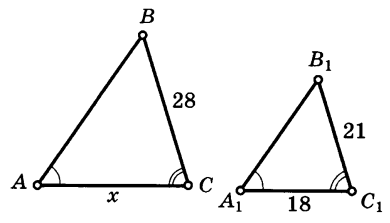
\includegraphics[align=t, width=1.5\linewidth]{../../../../exercises/lists/pics/G81M9L5-2}
		\end{minipage}
		\item 
		\begin{minipage}[t]{\bodywidth}
			Треугольники \( QMR \) и \( Q_1M_1R_1 \) подобны. Периметр треугольника \(  M_1Q_1R_1 \) равен \( 100 \).
		\end{minipage}
		\hspace{0.02\linewidth}
		\begin{minipage}[t]{\picwidth}
			% TODO: \usepackage{graphicx} required
			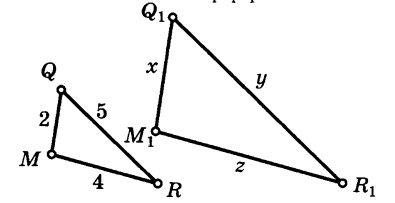
\includegraphics[align=t, width=1.5\linewidth]{../../../../exercises/lists/pics/G81M9L5-3}
		\end{minipage}
		\item 
		\begin{minipage}[t]{\bodywidth}
			Треугольники, изображенные на рисунке, подобны. Найдите стороны большего треугольника, если известно, что \( KL:LM:KM=6:7:5 \).
		\end{minipage}
		\hspace{0.02\linewidth}
		\begin{minipage}[t]{\picwidth}
			% TODO: \usepackage{graphicx} required
			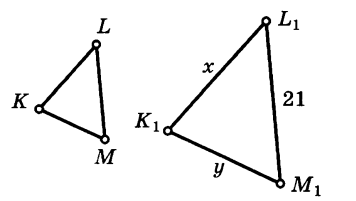
\includegraphics[align=t, width=1.5\linewidth]{../../../../exercises/lists/pics/G81M9L5-4}
		\end{minipage}
		\item
		\begin{minipage}[t]{\bodywidth}
			Найдите \( x \), \( y \).
		\end{minipage}
		\hspace{0.02\linewidth}
		\begin{minipage}[t]{\picwidth}
			% TODO: \usepackage{graphicx} required
			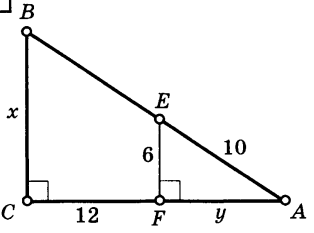
\includegraphics[align=t, width=\linewidth]{../../../../exercises/lists/pics/G81M9L5-5}
		\end{minipage}
		\item
		\begin{minipage}[t]{\bodywidth}
			Найдите \( x \), \( y \).
		\end{minipage}
		\hspace{0.02\linewidth}
		\begin{minipage}[t]{\picwidth}
			% TODO: \usepackage{graphicx} required
			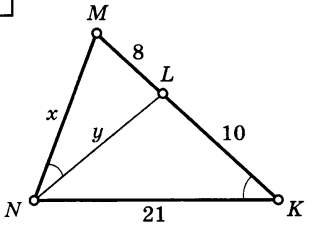
\includegraphics[align=t, width=\linewidth]{../../../../exercises/lists/pics/G81M9L5-6}
		\end{minipage}
		\item
		\begin{minipage}[t]{\bodywidth}
			Найдите \( x \), \( y \).
		\end{minipage}
		\hspace{0.02\linewidth}
		\begin{minipage}[t]{\picwidth}
			% TODO: \usepackage{graphicx} required
			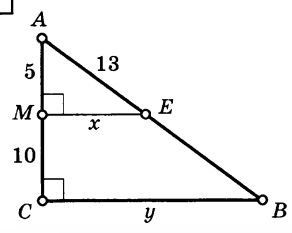
\includegraphics[align=t, width=\linewidth]{../../../../exercises/lists/pics/G81M9L5-7}
		\end{minipage}
		\item
		\begin{minipage}[t]{\bodywidth}
			Найдите \( x \), \( y \). Известно, что \( ON=12 \).
		\end{minipage}
		\hspace{0.02\linewidth}
		\begin{minipage}[t]{\picwidth}
			% TODO: \usepackage{graphicx} required
			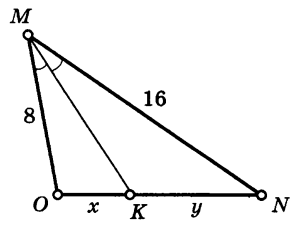
\includegraphics[align=t, width=\linewidth]{../../../../exercises/lists/pics/G81M9L5-8}
		\end{minipage}
		\item 
		\begin{minipage}[t]{\bodywidth}
			Укажите пары подобных треугольников и докажите их подобие.
		\end{minipage}
		\hspace{0.02\linewidth}
		\begin{minipage}[t]{\picwidth}
			% TODO: \usepackage{graphicx} required
			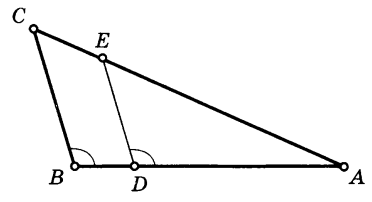
\includegraphics[align=t, width=\linewidth]{../../../../exercises/lists/pics/G81M9L5-9}
		\end{minipage}
		\item 
		\begin{minipage}[t]{\bodywidth}
			Треугольник \( KMN \) прямоугольный, \( KF \) его высота. Найдите пару подобных треугольников и докажите их подобие.
		\end{minipage}
		\hspace{0.02\linewidth}
		\begin{minipage}[t]{\picwidth}
			% TODO: \usepackage{graphicx} required
			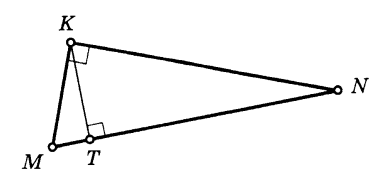
\includegraphics[align=t, width=\linewidth]{../../../../exercises/lists/pics/G81M9L5-10}
			
		\end{minipage}
		\item В треугольнике \( ABC \) на его медиане \( BM \) отмечена точка \( K \) так, что \( BK:KM=4:1 \). Прямая \( AK \) пересекает сторону \( BC \) в точке \( P \). Найдите отношение площади треугольника \( BKP \) к площади треугольника \( ABC \).
		\item 
		\begin{minipage}[t]{\bodywidth}
			На рисунке треугольник \( MOP \) --- равнобедренный, \( OP \) --- его основание, \( MK \) и \( OH \) --- высоты. Докажите, что треугольники \( MOK \) и \( MCH \) подобны и найдите \( CH \), если \( MH=6 \), \( PH=4 \), \( OP=12 \).
		\end{minipage}
		\hspace{0.02\linewidth}
		\begin{minipage}[t]{\picwidth}
			% TODO: \usepackage{graphicx} required
			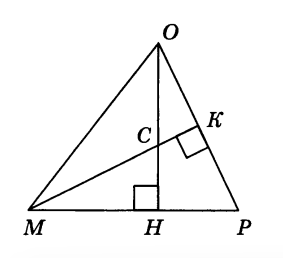
\includegraphics[align=t, width=\linewidth]{../../../../exercises/lists/pics/G81M9L5-1}
		\end{minipage}
			\item Средние линии треугольника относятся как \( 2 : 3 : 4 \), а периметр треугольника равен \( 45 \) см. Найдите стороны треугольника.
		\item Стороны треугольника равны \( 5 \) см, \( 3 \) см и \( 7 \) см. Найдите стороны подобного ему треугольника, периметр которого равен \( 105 \) см.
		\item Медианы треугольника АВС пересекаются в точке \( O \). Через точку \( O \) проведена прямая, параллельная стороне \( AC \) и пересекающая стороны \( AB \) и \( BC \) в точках \( E \) и \( F \) соответственно. Найдите \( EF \), если сторона \( AC \) равна \( 15 \) см.
		\item  У подобных треугольников сходственные стороны равны \( 7 \) см и \( 35 \) см. Площадь первого треугольника равна \( 27 \) см\( ^{2} \). Найдите площадь второго треугольника.
	\end{listofex}
\end{class}
%END_FOLD